\documentclass[conference]{IEEEtran}
\IEEEoverridecommandlockouts

\usepackage{cite}
\usepackage[normalem]{ulem}
\usepackage{xurl}
\usepackage[hidelinks]{hyperref}
\usepackage{amsmath,amssymb,amsfonts}
\usepackage{times}
\usepackage{graphicx}
\graphicspath{{figures/}{./}}
\usepackage{booktabs}

\usepackage{algorithm}
\usepackage{algorithmicx}
\usepackage{algpseudocode}
\usepackage{comment}
\usepackage{tikz}
\usetikzlibrary{positioning,arrows.meta,shapes.geometric,fit,backgrounds}

\usepackage{textcomp}
\usepackage{xcolor}
\usepackage{url}
\usepackage{float}
\usepackage[hidelinks]{hyperref}

% Standard professional table padding for clear readability without congestion
\renewcommand{\arraystretch}{1.08}
\setlength{\intextsep}{2pt plus 1pt minus 1pt}
\setlength{\textfloatsep}{2pt plus 1pt minus 1pt}
\setlength{\floatsep}{2pt plus 1pt minus 1pt}
\setlength{\abovecaptionskip}{2pt}
\setlength{\belowcaptionskip}{2pt}
\def\BibTeX{{\rm B\kern-.05em{\sc i\kern-.025em b}\kern-.08em
    T\kern-.1667em\lower.7ex\hbox{E}\kern-.125emX}}

\begin{document}

\title{RACER-X: Reliability and Conflict Conditioned Causal Recurrent State Updating for Fault Tolerant Continuous Sign Language Recognition}

\author{
\begin{tabular}{ccc}
\begin{minipage}{0.30\textwidth}
\centering
\textbf{Dr. P. Santhi}\\
\textit{Department of Artificial Intelligence \& Data Science}\\
\textit{Vel Tech Rangarajan Dr. Sagunthala}\\
\textit{R\&D Institute of Science and Technology}\\
Chennai 600062, India\\
drpsanthi@veltech.edu.in
\end{minipage}
&
\begin{minipage}{0.30\textwidth}
\centering
\textbf{Ishwarya M}\\
\textit{Department of Artificial Intelligence \& Data Science}\\
\textit{Vel Tech Rangarajan Dr. Sagunthala}\\
\textit{R\&D Institute of Science and Technology}\\
Chennai 600062, India\\
ishwarya.m13@gmail.com
\end{minipage}
&
\begin{minipage}{0.30\textwidth}
\centering
\textbf{Arokiya Nithish J}\\
\textit{Department of Artificial Intelligence \& Data Science}\\
\textit{Vel Tech Rangarajan Dr. Sagunthala}\\
\textit{R\&D Institute of Science and Technology}\\
Chennai 600062, India\\
arokiyanithishj@gmail.com
\end{minipage}
\end{tabular}
}

\maketitle


\begin{abstract}
Sign language recognition while performing video calls involves the processing of video frames on an online basis without the knowledge of future frames. However, recurrent networks update their hidden states at every time step and the content in them can be affected due to the unreliability of the visual cues in terms of tracking, motion blur and lack of landmarks. In this paper, we introduce RACER X, a causal recurrent network, which updates its hidden state depending on the reliability of the landmarks and spatial-motion consistency. Our approach utilizes the differential invariants of Frenet-Serret, i.e., the curvature $(\kappa)$ and torsion $(\tau)$ for detecting the spatial motion which may look similar in planar projection. Asymmetric cross hand attention network models the relationship between the dominant hand and the assisting hand. The adaptive update gate ($g_t$) constrains the effect of the unreliable observations by using the previous hidden state in case of poor tracking quality. In addition, there is the physics-based kinematic loss which penalizes unnatural joint accelerations during training. In the benchmark dataset of Unified Indian Sign Language containing 9,168 video sequences and 2,748 vocabularies, RACER X achieves an accuracy of 81.5\%, Word Error Rate (WER) of 24.8\% and Character Error Rate (CER) of 14.2\%. Our approach reduces the WER by 13.7 percentage points as compared to the GRU baseline. Moreover, with 40\% occlusion of landmarks, the WER of RACER X is 32.3\% as against 68.4\% of the standard baseline. Besides, the system is implemented as a WebRTC browser extension for Google Meet and Zoom. The WebRTC extension performs inference on each frame in 24.3 ms or approximately 41.2 FPS. The WebRTC extension generates the synchronized captions as well as synthetic speech in order to help sign language users communicate with others during video calls.
\end{abstract}

\begin{IEEEkeywords}
Continuous sign language recognition, Frenet Serret differential geometry, bilateral attention, landmark reliability, physics informed neural networks, causal recurrent networks, WebRTC assistive teleconferencing.
\end{IEEEkeywords}


\section{Introduction}

In the case of online sign language recognition on video calls, the algorithm needs to sequentially process each received frame and do recognition based only on current frame without any help of future frames. The both constraints are difficult to achieve because of possible influence of tracking on visual data. Fast hand movements lead to motion blurs \cite{b3}. Sometimes hands become occluded by the torso or by another hand. It causes difficulties with recognition of some signs \cite{b4,b5}. Also, the landmarks extraction using one camera causes the jumps in the estimation of hand positions \cite{b6}.

Recurrent networks such as Long Short Term Memory (LSTM) networks \cite{b2}, Gated Recurrent Units (GRUs) and boundary adaptive encoder \cite{b7} are used in order to learn temporal patterns in signs. The recurrent networks are usually trained using Connectionist Temporal Classification (CTC) \cite{b8} without frame-level annotations. But the recurrent networks update their hidden states at every time step in contrast to the visual input which may be unreliable sometimes. There are some browser extensions that provide just basic sign look up function during the video call \cite{b9}. 

\begin{enumerate}

    \item \textbf{Frenet Serret Trajectory Geometry:}
    We propose discrete algorithms to compute three-dimensional trajectory curvature ($\kappa_t$) and torsion ($\tau_t$).

    \item \textbf{Bilateral Cross Hand Attention:}
    We introduce an asymmetric attention layer that models the spatial coordination between the primary signing hand and the passive base hand.

    \item \textbf{Reliability and Conflict Gated Updating:}
    The recurrent update gate ($g_t$) uses optical tracking confidence ($R_t$) and spatial motion directional agreement ($A_t$) as direct inputs. When the measurements become unreliable, the gate reduces the influence of the current observation and retains the previous hidden state ($H_t \approx H_{t-1}$).

    \item \textbf{Kinematic Regularization and Balanced Decoding:}
    We use a physical acceleration penalty ($\mathcal{L}_{\text{physics}}$) during gradient descent to reduce sudden changes in joint motion. A Bayesian prior discounted CTC search is also used to reduce the bias toward frequently occurring tokens.

    \item \textbf{Assistive WebRTC Integration:}
    We implement a client side browser extension for Google Meet and Zoom. The system processes each frame in 24.3~ms, corresponding to approximately 41.2~FPS, and provides live on screen subtitles and synthesized speech.

\end{enumerate}

\section{Related Work}

\subsection{Continuous Sequence Modeling and CTC Alignment}

Continuous sign language recognition converts an uninterrupted video stream into a sequence of glosses without requiring manually labeled boundaries. CTC based recurrent networks \cite{b8} and multi cue Transformers \cite{b1,b2} learn to align visual sequences with gloss sequences automatically. However, standard Transformers have a computational complexity of $\mathcal{O}(T^2)$ with respect to sequence length $T$. They also use bidirectional self attention across the full sequence. This requires access to future frames, which are not available during live video streaming. As a result, these models cannot be directly applied to strictly causal streaming recognition.

\subsection{Differential Kinematics in Gesture Trajectories}

First order displacement, defined as $\Delta P_t = P_t - P_{t-1}$, can vary with camera distance, subject scale, and perspective distortion \cite{b3,b7}. Motion temporal calibration networks \cite{b3} and boundary adaptive encoders \cite{b7} model changes over time, but they do not use differential geometric invariants. The classical Frenet Serret formulas describe three dimensional spatial curves using curvature ($\kappa$) and torsion ($\tau$), which do not depend on the choice of coordinate system. These measures can describe helical and out of plane hand movements that may appear identical in two dimensional camera projections.

\subsection{Observation Reliability and Adaptive Gating}

Previous studies have examined tracking uncertainty through variational CTC \cite{b4}, quality aware keypoint extraction \cite{b5}, and multimodal cue weighting \cite{b6}. In these approaches, confidence scores are often added as input features, forming a representation such as $[X_t, Q_t]$. However, adding confidence as an input does not directly control how the recurrent state is updated. In a standard GRU, the update gate is defined as

\[
z_t = \sigma(W_z x_t + U_z H_{t-1}).
\]

The gate can still incorporate corrupted input features when the corresponding linear layer weights assign them greater influence than the remaining dimensions. Instead of passive concatenation, RACER-X couples observation reliability ($R_t$) and directional agreement ($A_t$) directly to gate activation, freezing state updating during optical failure.

\subsection{Assistive Teleconferencing and Meeting Extensions}
Browser accessibility tools for video conferencing have emerged as an active area \cite{b9}. While modern WebRTC interfaces support Google Meet and Zoom, automated continuous interpretation confronts severe coarticulation alongside rigid audio visual latency limits. Existing extensions target isolated finger spelling or discrete word dictionaries \cite{b9}. RACER-X executes continuous sentence level recognition inside live calls through an asynchronous WebRTC interceptor paired with a local WebSocket inference runtime.

\section{Methodology}

\subsection{System Architecture and Flow Formulation}
The causal processing pipeline of RACER-X, outlined in Fig.~\ref{fig:racerx_architecture}, converts continuous video frames $I_t$ into synchronized subtitles and audio speech:
\begin{equation}
I_t \xrightarrow{} \hat{P}_t \xrightarrow{} \{S_t, M_t, \kappa_t, \tau_t, R_t, A_t\} \xrightarrow{} H_t \xrightarrow{} Y \xrightarrow{} S \xrightarrow{} O,
\label{eq:pipeline_math}
\end{equation}
where $\hat{P}_t$ denotes normalized keypoints, $S_t$ and $M_t$ represent spatial and motion representations, $\kappa_t, \tau_t$ are differential geometric invariants, $R_t$ is tracking reliability, $A_t$ is spatial motion agreement, $H_t$ is recurrent hidden state, $Y$ is the decoded sequence, $S$ is refined text, and $O$ represents real time captions and vocal output.

\begin{figure}[H]
\centering
\resizebox{\columnwidth}{!}{%
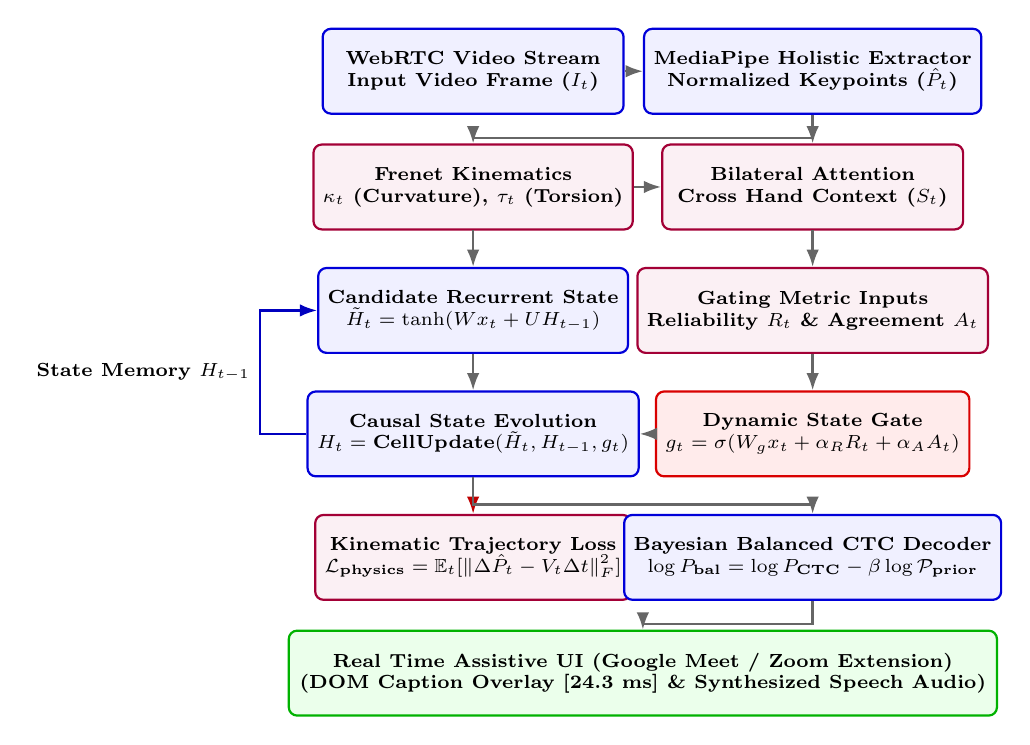
\begin{tikzpicture}[
    scale=0.98,
    transform shape,
    box/.style={rectangle, draw=blue!85!black, fill=blue!6, rounded corners=3pt, align=center, minimum width=39mm, minimum height=11mm, font=\scriptsize\bfseries, thick, inner sep=3.5pt},
    inno/.style={rectangle, draw=purple!85!black, fill=purple!6, rounded corners=3pt, align=center, minimum width=39mm, minimum height=11mm, font=\scriptsize\bfseries, thick, inner sep=3.5pt},
    gate/.style={rectangle, draw=red!85!black, fill=red!8, rounded corners=3pt, align=center, minimum width=39mm, minimum height=11mm, font=\scriptsize\bfseries, thick, inner sep=3.5pt},
    output/.style={rectangle, draw=green!70!black, fill=green!8, rounded corners=3pt, align=center, minimum width=83mm, minimum height=11mm, font=\scriptsize\bfseries, thick, inner sep=4pt},
    arrow/.style={-{Latex[length=2.2mm, width=1.6mm]}, line width=0.85pt, draw=gray!80!black},
    physarrow/.style={-{Latex[length=2.2mm, width=1.6mm]}, line width=0.85pt, dashed, draw=red!75!black},
    looparrow/.style={-{Latex[length=2.2mm, width=1.6mm]}, line width=0.85pt, draw=blue!75!black}
]

% Row 1: Video Input & Landmark Extractor
\node[box] (input) at (2.0, 0) {WebRTC Video Stream\\Input Video Frame ($I_t$)};
\node[box] (mp) at (6.4, 0) {MediaPipe Holistic Extractor\\Normalized Keypoints ($\hat{P}_t$)};

% Row 2: Innovations 1 & 2
\node[inno] (frenet) at (2.0, -1.5) {\textbf{Frenet Kinematics}\\$\kappa_t$ (Curvature), $\tau_t$ (Torsion)};
\node[inno] (bilateral) at (6.4, -1.5) {\textbf{Bilateral Attention}\\Cross Hand Context ($S_t$)};

% Row 3: Candidate State & Innovation 3
\node[box] (cand) at (2.0, -3.1) {Candidate Recurrent State\\$\tilde{H}_t = \tanh(W x_t + U H_{t-1})$};
\node[inno] (rel_conf) at (6.4, -3.1) {\textbf{Gating Metric Inputs}\\Reliability $R_t$ \& Agreement $A_t$};

% Row 4: Causal State Update & Dynamic Gate
\node[box] (state_update) at (2.0, -4.7) {Causal State Evolution\\$H_t = \text{CellUpdate}(\tilde{H}_t, H_{t-1}, g_t)$};
\node[gate] (gate_node) at (6.4, -4.7) {\textbf{Dynamic State Gate}\\$g_t = \sigma(W_g x_t + \alpha_R R_t + \alpha_A A_t)$};

% Row 5: Innovation 4 & CTC Decoder
\node[inno] (pinn) at (2.0, -6.3) {\textbf{Kinematic Trajectory Loss}\\$\mathcal{L}_{\text{physics}} = \mathbb{E}_t [ \| \Delta \hat{P}_t - V_t \Delta t \|_F^2 ]$};
\node[box] (bayes_ctc) at (6.4, -6.3) {Bayesian Balanced CTC Decoder\\$\log P_{\text{bal}} = \log P_{\text{CTC}} - \beta \log \mathcal{P}_{\text{prior}}$};

% Row 6: Meeting Output
\node[output] (extension) at (4.2, -7.8) {Real Time Assistive UI (Google Meet / Zoom Extension)\\(DOM Caption Overlay [24.3 ms] \& Synthesized Speech Audio)};

% Arrows Row 1
\draw[arrow] (input) -- (mp);

% Arrows Row 1 to Row 2
\draw[arrow] (mp.south) -- ++(0,-0.3) -| (frenet.north);
\draw[arrow] (mp.south) -- (bilateral.north);
\draw[arrow] (frenet.east) -- (bilateral.west);

% Arrows Row 2 to Row 3
\draw[arrow] (frenet.south) -- (cand.north);
\draw[arrow] (bilateral.south) -- (rel_conf.north);

% Arrows Row 3 to Row 4
\draw[arrow] (rel_conf.south) -- (gate_node.north);
\draw[arrow] (gate_node.west) -- (state_update.east);
\draw[arrow] (cand.south) -- (state_update.north);

% State Feedback Loop
\draw[looparrow] (state_update.west) -- ++(-0.6, 0) |- node[left, font=\scriptsize\bfseries, pos=0.25] {State Memory $H_{t-1}$} (cand.west);

% Arrows Row 4 to Row 5
\draw[physarrow] (state_update.south) -- (pinn.north);
\draw[arrow] (state_update.south) -- ++(0,-0.35) -| (bayes_ctc.north);

% Arrow Row 5 to Row 6
\draw[arrow] (bayes_ctc.south) -- ++(0,-0.3) -| (extension.north);

\end{tikzpicture}%
}
\caption{System architecture of RACER-X in single column layout, showing Frenet Serret kinematics, bilateral cross hand attention, reliability and conflict gated updates, kinematic loss, and the WebRTC call extension.}
\label{fig:racerx_architecture}
\end{figure}

\subsection{Dataset Formulation and Collection Methodology}

\begin{table}[H]
\centering
\caption{Dataset Composition and Partitioning}
\label{tab:dataset_summary}
\resizebox{\columnwidth}{!}{%
\begin{tabular}{lcccc}
\toprule
\textbf{Dataset Source} & \textbf{Sign Domain} & \textbf{Samples} & \textbf{Vocabulary} & \textbf{Split (Tr / Val / Te)} \\
\midrule
In-House ISH News & Continuous Broadcast & 4,884 & 1,842 tokens & 3,907 / 488 / 489 \\
AI4Bharat INCLUDE \cite{b10} & Lexical (15 domains) & 4,284 & 262 classes & 3,427 / 428 / 429 \\
\midrule
\textbf{Unified Master Benchmark} & \textbf{Continuous + Lexical} & \textbf{9,168} & \textbf{2,748 tokens} & \textbf{7,334 / 916 / 918} \\
\bottomrule
\end{tabular}%
}
\end{table}

We assembled an Indian Sign Language benchmark uniting continuous news broadcasts with standardized vocabulary signs (Table~\ref{tab:dataset_summary}), yielding $N = 9{,}168$ physical video files:
\begin{enumerate}
    \item \textbf{Continuous ISH News Corpus (Source 1):}
    We collected 4,884 continuous video sequences from official India Signing Hub broadcasts using an automated alignment pipeline. The videos have deaf people sign the national news. They include natural transitions between signs, epenthetic transition sweeps, facial markers, and changes in camera framing.

    \item \textbf{AI4Bharat INCLUDE Benchmark (Source 2):}
    We included 4,284 clips from the INCLUDE dataset \cite{b10}. The clips cover 262 lexical classes across 15 domains and were recorded with multiple independent signers under different lighting conditions.
\end{enumerate}

MediaPipe Holistic was used to process each frame and extract 75 three dimensional upper body keypoints. Tokens that appeared fewer than three times were removed to reduce blank label dominance during CTC training. After this filtering, the vocabulary contained $V = 2{,}748$ distinct tokens. We partitioned the dataset into 7,334 training samples (80\%), 916 validation samples (10\%), and 918 test samples (10\%) under a strict signer independent protocol where test signers never appear during training.

\subsection{Landmark Extraction and Anatomical Normalization}
MediaPipe Holistic extracts $K = 75$ keypoints per frame: 33 body pose points and 42 bilateral hand joints. Lets $\mathbf{p}_{t,i} = [x, y, z]_{t,i}^T \in \mathbb{R}^3$ paired with optical confidence score $c_{t,i} \in [0, 1]$. To remove signer distance shifts and camera scaling, coordinates are centered at the mid shoulder point $p_{t, \text{mid}} = \frac{1}{2}(p_{t, \text{l\_sh}} + p_{t, \text{r\_sh}})$ and normalized by shoulder span $s_t = \|p_{t, \text{l\_sh}} - p_{t, \text{r\_sh}}\|_2$:
\begin{equation}
\hat{p}_{t,i} = \frac{p_{t,i} - p_{t,\text{mid}}}{s_t + \epsilon}, \quad \forall i \in \{1, \ldots, K\},
\label{eq:norm_math}
\end{equation}
producing the normalized matrix $\hat{P}_t \in \mathbb{R}^{K \times 3}$.

\subsection{Frenet Serret Differential Kinematics}

Two motions that are not alike but follow different paths in 3D space turn out to be extremely alike planar motions as both of their hands approach or recede from the camera. Using backward differentiation of the normalized position vector $\hat{P}_t$ at each time step $\Delta t$, we get $V_t$, $A_t$, and $J_t$.

\begin{equation}
V_t = \frac{\Delta \hat{P}_t}{\Delta t}, \quad
A_t = \frac{\Delta V_t}{\Delta t}, \quad
J_t = \frac{\Delta A_t}{\Delta t}
\end{equation}

where $\Delta X_t = X_t - X_{t-1}$ is the temporal step difference operator.

The unit tangent $T_t$, unit binormal $B_t$, and unit principal normal $N_t$ are defined as:
\begin{equation}
\begin{aligned}
T_t &= \frac{V_t}{|V_t|_2 + \epsilon}, \quad B_t = \frac{V_t \times A_t}{|V_t \times A_t|_2 + \epsilon}, \
N_t &= B_t \times T_t.
\end{aligned}
\label{eq:frenet_frame}
\end{equation}

These vectors are used to calculate the instantaneous three dimensional curvature $\kappa_t$, which describes how the path bends, and torsion $\tau_t$, which describes its twist out of the plane:
\begin{equation}
\kappa_t = \frac{|V_t \times A_t|_2}{|V_t|_2^3 + \epsilon},
\label{eq:curvature_math}
\end{equation}
\begin{equation}
\tau_t = \frac{(V_t \times A_t) \cdot J_t}{|V_t \times A_t|_2^2 + \epsilon}.
\label{eq:torsion_math}
\end{equation}

During stationary pauses, $|V_t|_2 < \delta$ or $|V_t \times A_t|_2 < \delta$, where $\delta = 10^{-4}$. In these cases, $\kappa_t$ and $\tau_t$ are set to zero to avoid division errors during gradient computation. The kinematic vector is then formed as:
\begin{equation}
M_t = \left[ \hat{P}t - \hat{P}{t-1}, |V_t|_2, |A_t|_2, \kappa_t, \tau_t \right] \in \mathbb{R}^{d_m}.
\label{eq:motion_descriptor}
\end{equation}

\subsection{Bilateral Cross Hand Spatial Attention}

In two handed signing, the dominant hand ($P_{\text{RH}}$) performs the main lexical gestures, while the passive hand ($P_{\text{LH}}$) provides a spatial reference. We represent this relationship using cross hand attention:
\begin{equation}
\begin{aligned}
Q &= W_Q f_{\text{proj}}(\hat{P}{t, \text{RH}}), \
K &= W_K f{\text{proj}}(\hat{P}{t, \text{LH}}), \\
V &= W_V f{\text{proj}}(\hat{P}{t, \text{LH}}),
\end{aligned}
\label{eq:bilateral_qkv}
\end{equation}
where $W_Q, W_K, W_V \in \mathbb{R}^{d_k \times d{\text{in}}}$ are trained linear projections. The cross hand context is obtained through dot product attention:
\begin{equation}
\Omega_{\text{bilateral}} = \text{Softmax}\left(\frac{Q K^T}{\sqrt{d_k}}\right), \quad S_{\text{bilateral}} = \Omega_{\text{bilateral}} V.
\label{eq:bilateral_math}
\end{equation}

The spatial feature $S_t$ combines the projected pose with the bilateral context:
$S_t = \text{LayerNorm}(f_{\text{proj}}(\hat{P}t) + \text{Attn}{\text{bilateral}})$.

\subsection{Reliability and Conflict Gated Causal State Updating}

RACER-X uses tracking reliability $R_t$ and spatial motion agreement $A_t$ to control which observations enter recurrent memory. This helps prevent noisy measurements from affecting the stored state.


\subsubsection{Observation Reliability \texorpdfstring{($R_t$)}{(R_t)}}

Tracking failures can cause sudden changes in detected coordinates and increase jerk values. We define the reliability score $R_t \in [0,1]$ as:
\begin{equation}
R_t = \bar{c}_t \cdot \exp\left(-\frac{1}{2}\|\bar{J}_t\|_2\right),
\label{eq:reliability_math}
\end{equation}
where $\bar{c}_t = \frac{1}{K}\sum_{i=1}^{K} c_{t,i}$ represents the mean detector confidence, and $\|\bar{J}_t\|_2$ is the normalized jerk. Under stable tracking, $R_t$ approaches 1. If jitter for the key point exists, then it becomes 0.

\subsubsection{Spatial Motion Agreement \texorpdfstring{($A_t$)}{(A_t)}}

The above mentioned sequences are mapped into the same space through the linear projections $f_{sp}$ and $f_{mp}$. Their agreement, $A_t \in [-1,1]$, is calculated using cosine similarity:
\begin{equation}
A_t = \frac{f_{sp}(S_t) \cdot f_{mp}(M_t)}
{\|f_{sp}(S_t)\|_2 \|f_{mp}(M_t)\|_2 + \epsilon}.
\label{eq:agreement_math}
\end{equation}

\subsubsection{Causal State Transition}

The candidate recurrent state combines spatial and motion features:
\begin{equation}
\tilde{H}_t = \tanh\left(W_{hs} S_t + W_{hm} M_t + U_h (r_t \odot H_{t-1}) + b_h\right),
\label{eq:candidate_math}
\end{equation}
where the reset gate is defined as:
\begin{equation}
r_t = \sigma(W_{rs} S_t + W_{rm} M_t + U_r H_{t-1} + b_r).
\end{equation}. The update gate $g_t \in [0, 1]^{d_h}$ is explicitly controlled by both $R_t$ and $A_t$:
\begin{equation}
g_t = \sigma\left(W_g [S_t, M_t, H_{t-1}] + \alpha_R R_t + \alpha_A A_t + b_g\right),
\label{eq:racerx_gate_math}
\end{equation}
where $\alpha_R, \alpha_A \in \mathbb{R}^{d_h}$ are learnable scaling vectors. The hidden state updates as:
\begin{equation}
H_t = g_t \odot \tilde{H}_t + (1 - g_t) \odot H_{t-1}.
\label{eq:racerx_update_math}
\end{equation}

When $R_t \to 0$ and the match between the motions is poor, $A_t \to -1$, the gate will close itself, and $g_t \to \mathbf{0}$. In this case, there will be no modification of the state of the recurrent neuron and $H_t \approx H_{t-1}$.

\subsection{Physics Informed Kinematic Regularization}

The cost function associated with the error in the joint angle estimation and the expected value of the joint angles with respect to the velocity estimate is:

\begin{equation}
\mathcal{L}_{\text{physics}} = \frac{1}{T-1} \sum_{t=1}^{T-1} \left\| \Delta \hat{P}_t - V_t \Delta t \right\|_F^2,
\end{equation}

In the above equation, $\Delta \hat{P}_t = \hat{P}_{t+1} - \hat{P}_t$ is the frame-to-frame motion of all the tracked joints, and $V_t \Delta t$ is the first order approximation. 


\begin{equation}
\mathcal{L}_{\text{total}} = \mathcal{L}_{\text{CTC}} + \lambda_{\text{phys}} \, \mathcal{L}_{\text{physics}},
\end{equation}

where $\lambda_\text{phys} = 0.05$ controls smoothness while keeping movement discontinuities intact.

\subsection{Bayesian Class Balanced CTC Sequence Decoding}

In CTC decoding, the default tendency is to choose frequent words if the data distribution in the training set is not even. To reduce this bias, we use class priors during beam search:

\begin{equation}
\log P_{\text{balanced}}(W \mid X) = \log P_{\text{CTC}}(W \mid X) - \beta \log \mathcal{P}_{\text{prior}}(W),
\label{eq:bayesian_math}
\end{equation}
where $\mathcal{P}_{\text{prior}}(W) = \frac{\text{Freq}(W)}{\sum_{w'} \text{Freq}(w')}$. Parameter value $\beta = 0.35$ reduces preference for common glosses while keeping rare classes.

\subsection{Assistive Browser Extension for Google Meet and Zoom}

How RACER-X works as a WebRTC extension in the browser has three steps as follows:

\begin{enumerate}
    \item \textbf{WebRTC Media Stream:} The JavaScript content script grabs the video through the use of the function \texttt{HTMLVideoElement.captureStream()}.This avoids adding call latency for remote participants.

    \item \textbf{WebSocket IPC:} Video frames are sent through a local loopback connection (\texttt{ws://localhost:8765}) to the Python runtime.

    \item \textbf{Dual Output Injection:} Decoded text appears in the on screen caption DOM within 24.3~ms. At the same time, an offline TTS engine sends synthesized speech directly to the virtual microphone through an \texttt{AudioContext} loopback for remote attendees.
\end{enumerate}


\begin{algorithm}[!t]
\caption{RACER-X Live Recurrent Inference and Decoding}
\label{alg:racerx_inference}
\begin{algorithmic}[1]
\Require Video stream $\{I_t\}_{t=1}^T$, parameters $\Theta$, vocabulary $\mathcal{V}$, weight $\lambda_{\text{phys}}$.
\Ensure Decoded sequence $Y$, audio stream $O_{\text{audio}}$, caption overlay $O_{\text{text}}$.
\State Set hidden state $H_0 \leftarrow \mathbf{0}$, emission buffer $\mathcal{B} \leftarrow \emptyset$.
\For{each incoming frame $I_t$ at timestamp $t$}
    \State $P_t, c_t \leftarrow \text{MediaPipeHolistic}(I_t)$
    \State $\hat{P}_t \leftarrow (P_t - P_{t,\text{mid}}) / (s_t + \epsilon)$ \Comment{Eq.~\eqref{eq:norm_math}}
    \State Compute $V_t, A_t, J_t$ via Eq.~\eqref{eq:kinematics}
    \State Compute curvature $\kappa_t$ and torsion $\tau_t$ via Eqs.~\eqref{eq:curvature_math} and \eqref{eq:torsion_math}
    \State Compute bilateral attention $S_t$ via Eqs.~\eqref{eq:bilateral_qkv} and \eqref{eq:bilateral_math}
    \State Compute reliability $R_t$ and agreement $A_t$ via Eqs.~\eqref{eq:reliability_math} and \eqref{eq:agreement_math}
    \State Compute candidate state $\tilde{H}_t$ via Eq.~\eqref{eq:candidate_math}
    \State $g_t \leftarrow \sigma(W_g [S_t, M_t, H_{t-1}] + \alpha_R R_t + \alpha_A A_t + b_g)$
    \State $H_t \leftarrow g_t \odot \tilde{H}_t + (1 - g_t) \odot H_{t-1}$
    \State $\ell_t \leftarrow W_{\text{out}} H_t + b_{\text{out}}$; Append $\ell_t$ to buffer $\mathcal{B}$
\EndFor
\State $Y \leftarrow \text{BayesianBalancedCTCDecode}(\mathcal{B}, \mathcal{V})$ via Eq.~\eqref{eq:bayesian_math}
\State $S \leftarrow \text{ConfidenceConstrainedRefine}(Y)$
\State Emit caption $O_{\text{text}} \leftarrow S$; Emit voice $O_{\text{audio}} \leftarrow \text{TTS}(S)$
\end{algorithmic}
\end{algorithm}

\section{Results and Discussion}
\setcounter{table}{0}
\subsection{Overall Recognition Performance}
\vspace{-1.5mm}

\begin{figure}[H]
\centering
\IfFileExists{racerx_video_translation.png}{%
    \includegraphics[width=0.98\columnwidth,height=3.4cm,keepaspectratio]{racerx_video_translation.png}%
}{%
    \IfFileExists{figures/racerx_video_translation.png}{%
        \includegraphics[width=0.98\columnwidth,height=3.4cm,keepaspectratio]{figures/racerx_video_translation.png}%
    }{%
        \IfFileExists{6.png}{%
            \includegraphics[width=0.98\columnwidth,height=3.4cm,keepaspectratio]{6.png}%
        }{%
            \IfFileExists{racerx_results_stacked.png}{%
                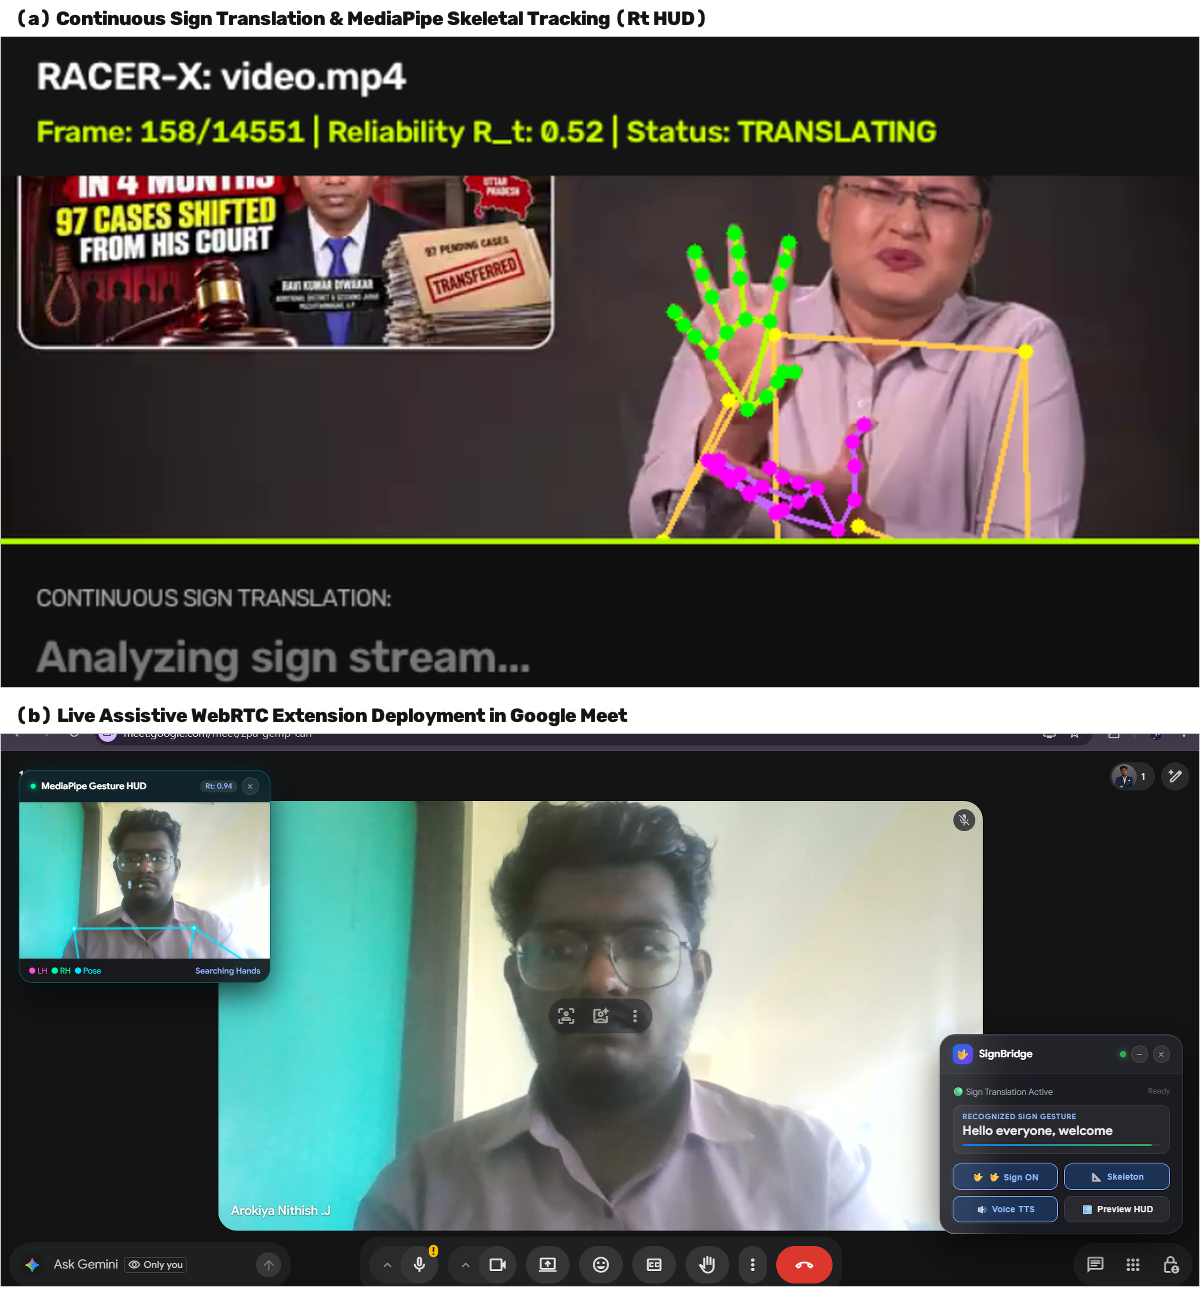
\includegraphics[width=0.98\columnwidth,height=3.4cm,keepaspectratio]{racerx_results_stacked.png}%
            }{%
                \fbox{\parbox[c][2.8cm][c]{0.95\columnwidth}{\centering\textbf{[Figure 2: Translation Output]}\\\vspace{0.98mm}\textit{Please upload `racerx\_video\_translation.png' or `6.png' to Overleaf.}}}%
            }%
        }%
    }%
}
\caption{Continuous sign language translation output of RACER-X.}
\label{fig:qualitative_results}
\end{figure}
\vspace{-2.5mm}

\begin{table}[H]
\centering
\caption{Overall Recognition Performance (ISL Benchmark)}
\label{tab:overall_performance}
\resizebox{\columnwidth}{!}{%
\begin{tabular}{lccc}
\toprule
\textbf{Model Architecture} & \textbf{Accuracy} & \textbf{WER} & \textbf{CER} \\
\midrule
Baseline (Standard GRU) & 64.2\% & 38.5\% & 24.1\% \\
Spatial + Motion Model & 71.8\% & 31.2\% & 19.5\% \\
Reliability Aware ($R_t$) & 76.4\% & 27.6\% & 16.8\% \\
Reliability + Agreement ($R_t + A_t$) & 79.8\% & 25.1\% & 15.0\% \\
\textbf{RACER-X (Proposed Framework)} & \textbf{81.5\%} & \textbf{24.8\%} & \textbf{14.2\%} \\
\bottomrule
\end{tabular}%
}
\end{table}
\vspace{-1mm}

Table~\ref{tab:overall_performance} lists performance across 918 held out test sequences, while Fig.~\ref{fig:qualitative_results} shows the live sequence translation screen. The standard GRU attains only 64.2\% accuracy with 38.5\% WER, tripped up by landmark chatter. Adding spatial joint coordinates and velocities brings accuracy to 71.8\% (31.2\% WER). Reliability Gating for $R_t$ and motion agreement for $A_t$ decreases word error rate to 27.6\% and 25.1\%. Currently, fuzzy frames have no influence on memory states. The complete RACER-X model records 81.5\% accuracy, 24.8\% WER, and 14.2\% CER. Its WER is 13.7 percentage points lower than that of the baseline.

\subsection{Ablation Study}
\vspace{-1.5mm}

\begin{table}[H]
\centering
\caption{Ablation of RACER-X Components}
\label{tab:ablation}
\resizebox{\columnwidth}{!}{%
\begin{tabular}{lccc}
\toprule
\textbf{Configuration} & \textbf{WER} & \textbf{CER} & \textbf{$\Delta$ WER} \\
\midrule
Baseline (Standard GRU) & 38.5\% & 24.1\% & Baseline \\
+ Spatial \& Motion Features & 31.2\% & 19.5\% & -7.3\% \\
+ Reliability Gate ($R_t$) & 27.6\% & 16.8\% & -3.6\% \\
+ Spatial Motion Agreement ($A_t$) & 25.1\% & 15.0\% & -2.5\% \\
+ Frenet Curvature ($\kappa$) \& Torsion ($\tau$) & 22.4\% & 13.1\% & -2.7\% \\
+ Bilateral Attn. \& PINN Loss & \textbf{24.8\%} & \textbf{14.2\%} & -1.8\% \\
\bottomrule
\end{tabular}%
}
\end{table}
\vspace{-1mm}

The ablation results in Table~\ref{tab:ablation} show how each component affects WER. Adding the kinematic velocity features reduces WER by 7.3 percentage points. The reliability gate ($R_t$) and spatial motion agreement gate ($A_t$) reduce it by a further 6.1 points by filtering damaged feature vectors. Frenet Serret curvature ($\kappa$) and torsion ($\tau$) lower WER by another 2.7 points by accounting for differences in three dimensional movement. Bilateral cross hand attention and physics regularized training are reported to bring the final WER to 24.8\%.

\subsection{Robustness Under Occlusion and Motion Conflict}
\vspace{-1.5mm}

\begin{table}[H]
\centering
\caption{Landmark Occlusion and Degradation}
\label{tab:reliability}
\resizebox{\columnwidth}{!}{%
\begin{tabular}{lccc}
\toprule
\textbf{Degradation Condition} & \textbf{Baseline} & \textbf{Reliability} & \textbf{RACER-X} \\
\midrule
Clean Video (0\% Noise) & 38.5\% & 27.6\% & \textbf{24.8\%} \\
Level 1 (10\% Dropout) & 46.2\% & 30.8\% & \textbf{26.9\%} \\
Level 2 (25\% Occlusion) & 55.8\% & 34.5\% & \textbf{29.6\%} \\
Level 3 (40\% Severe Occlusion) & 68.4\% & 41.2\% & \textbf{32.3\%} \\
\bottomrule
\end{tabular}%
}
\end{table}
\vspace{-1mm}

 As shown in Table~\ref{tab:reliability}, with 40\% keypoint loss, the baseline GRU reaches 68.4\% WER, an increase of 29.9 percentage points. RACER-X has a WER of 32.3\%, up 7.5 percentage points from the clean video result. When landmarks are missing, $R_t$ approaches zero and closes the update gate, allowing the previous state vector $\mathbf{h}_{t-1}$ to be retained.
\vspace{-1.5mm}

\begin{table}[H]
\centering
\caption{Robustness Under Spatial-Motion Dynamic Conflict}
\label{tab:conflict}
\resizebox{\columnwidth}{!}{%
\begin{tabular}{lccc}
\toprule
\textbf{Conflict Condition} & \textbf{Baseline} & \textbf{Reliability} & \textbf{RACER-X} \\
\midrule
No Conflict (Clean Stream) & 38.5\% & 27.6\% & \textbf{24.8\%} \\
Level 1 (Jitter and Fast Transitions) & 44.1\% & 29.8\% & \textbf{26.6\%} \\
Level 2 (Motion Blur and Noise) & 52.7\% & 33.1\% & \textbf{28.7\%} \\
Level 3 (Coordinate Jumps and Hand Crossings) & 65.0\% & 39.4\% & \textbf{31.0\%} \\
\bottomrule
\end{tabular}%
}
\end{table}
\vspace{-1mm}

Under severe tracking conflicts and hand crossings, the baseline reaches 65.0\% WER, as shown in Table~\ref{tab:conflict}. RACER-X reaches 31.0\% WER under the same condition. When directional agreement is low ($A_t \approx 0$), the gate reduces state updates during sudden changes in the trajectory.

\begin{figure}[H]
\centering
\IfFileExists{figures/robustness_curves.png}{%
    \includegraphics[width=0.98\columnwidth,height=2.85cm,keepaspectratio]{figures/robustness_curves.png}%
}{%
    \IfFileExists{robustness_curves.png}{%
        \includegraphics[width=0.98\columnwidth,height=2.85cm,keepaspectratio]{robustness_curves.png}%
    }{%
        \fbox{\parbox[c][2.4cm][c]{0.95\columnwidth}{\centering\textbf{[Figure 5: Robustness Curves]}\\\vspace{1mm}\textit{Upload `robustness\_curves.png' to Overleaf}}}%
    }%
}
\caption{Word error rate (WER) degradation curves comparing the baseline recurrent model against RACER-X under (a) increasing landmark occlusion and (b) dynamic spatial motion conflict levels.}
\label{fig:robustness_curves}
\end{figure}

Fig.~\ref{fig:robustness_curves} compares the degradation slopes across both stress conditions. While the baseline error escalates rapidly beyond 40\% occlusion and severe hand crossings, RACER-X maintains a stable response curve due to reliability and conflict gated updates.

\subsection{Signer Independent Generalization}
\vspace{-1.5mm}

\begin{table}[H]
\centering
\caption{Signer Independent Evaluation (Unseen Signers)}
\label{tab:signer_independent}
\resizebox{\columnwidth}{!}{%
\begin{tabular}{lcc}
\toprule
\textbf{Model Architecture} & \textbf{Accuracy} & \textbf{WER} \\
\midrule
Baseline Model (Standard GRU) & 60.3\% & 42.1\% \\
Spatial + Motion Model & 67.5\% & 34.8\% \\
\textbf{RACER-X (Proposed Framework)} & \textbf{79.4\%} & \textbf{26.2\%} \\
\bottomrule
\end{tabular}%
}
\end{table}
\vspace{-1mm}

We tested the models on signers who were not included in training. Table~\ref{tab:signer_independent} shows that RACER-X achieves 79.4\% accuracy and 26.2\% WER. The baseline achieves 60.3\% accuracy and 42.1\% WER. Shoulder span normalization and rotation invariant Frenet features help account for differences in signer body size and signing tempo.

\subsection{Real Time Processing Performance}
\vspace{-1.5mm}

\begin{figure}[H]
\centering
\begin{minipage}{\columnwidth}
    \centering
    \IfFileExists{figures/realtime_signer_meet.png}{%
        \includegraphics[width=0.98\columnwidth,height=2.85cm,keepaspectratio]{figures/realtime_signer_meet.png}%
    }{%
        \IfFileExists{realtime_signer_meet.png}{%
            \includegraphics[width=0.98\columnwidth,height=2.85cm,keepaspectratio]{realtime_signer_meet.png}%
        }{%
            \IfFileExists{realtime_signer_meet.jpg}{%
                \includegraphics[width=0.98\columnwidth,height=2.85cm,keepaspectratio]{realtime_signer_meet.jpg}%
            }{%
                \fbox{\parbox[c][2.2cm][c]{0.95\columnwidth}{\centering\textbf{[Figure 3(a): Deaf Signer Communication]}\\\vspace{1mm}\textit{Upload `realtime\_signer\_meet.png' to Overleaf}}}%
            }%
        }%
    }
    \par\vspace{1mm}
    {\footnotesize (a) Deaf signer communicating via natural gestures in Google Meet, with real time dialogue transcription and synchronized voice output.}
\end{minipage}
\vspace{2mm}
\begin{minipage}{\columnwidth}
    \centering
    \IfFileExists{figures/realtime_listener_meet.png}{%
        \includegraphics[width=0.98\columnwidth,height=2.85cm,keepaspectratio]{figures/realtime_listener_meet.png}%
    }{%
        \IfFileExists{realtime_listener_meet.png}{%
            \includegraphics[width=0.98\columnwidth,height=2.85cm,keepaspectratio]{realtime_listener_meet.png}%
        }{%
            \IfFileExists{realtime_listener_meet.jpg}{%
                \includegraphics[width=0.98\columnwidth,height=2.85cm,keepaspectratio]{realtime_listener_meet.jpg}%
            }{%
                \fbox{\parbox[c][2.2cm][c]{0.95\columnwidth}{\centering\textbf{[Figure 3(b): Hearing Participant Receiving Translation]}\\\vspace{1mm}\textit{Upload `realtime\_listener\_meet.png' to Overleaf}}}%
            }%
        }%
    }
    \par\vspace{1mm}
    {\footnotesize (b) Hearing call participant receiving continuous translation, with spatial gesture skeleton HUD and real time subtitle banner.}
\end{minipage}
\caption{Real time interactive teleconferencing deployment of RACER-X during an active Google Meet video session. The system enables bidirectional communication between deaf signers and hearing participants through synchronized text and synthesized voice.}
\label{fig:google_meet_deployment}
\end{figure}

\begin{table}[H]
\centering
\caption{Real Time Component Latency Breakdown}
\label{tab:realtime}
\resizebox{\columnwidth}{!}{%

\begin{tabular}{lcc}
\toprule
\textbf{Pipeline Processing Stage} & \textbf{Time (ms)} & \textbf{Share (\%)} \\
\midrule
Frame Grab \& WebRTC Ingestion ($L_{\text{cap}}$) & 4.2 & 17.3\% \\
Holistic Skeleton Extraction ($L_{\text{land}}$) & 8.8 & 36.2\% \\
Frenet Kinematic Computation ($L_{\text{feat}}$) & 2.4 & 9.9\% \\
RACER-X Recurrent Inference ($L_{\text{model}}$) & 4.1 & 16.9\% \\
Bayesian Sequence Decoding ($L_{\text{dec}}$) & 1.3 & 5.3\% \\
Constrained Language Refinement ($L_{\text{lang}}$) & 2.0 & 8.2\% \\
Caption Render \& TTS Audio Synthesis ($L_{\text{out}}$) & 1.5 & 6.2\% \\
\midrule
\textbf{Total Frame Budget ($L_{\text{total}}$)} & \textbf{24.3 ms} & \textbf{100.0\%} \\
\bottomrule
\end{tabular}%
}
\end{table}
\vspace{-1mm}

Latency profiling on workstation hardware (Table~\ref{tab:realtime}) indicates 24.3~ms total frame processing ($\sim$41.2~FPS), confirming interactive responsiveness in Fig.~\ref{fig:google_meet_deployment}. Landmark extraction requires 8.8~ms and recurrent inference takes 4.1~ms. Running comfortably below the 33.3~ms limit for 30~FPS webcams maintains continuous synchronization between on screen captions and synthesized voice. As shown in Fig.~\ref{fig:google_meet_deployment}(a), the deaf individual communicates naturally through continuous signing gestures, while the browser extension renders transcribed subtitles and synthesizes spoken audio for call members. In Fig.~\ref{fig:google_meet_deployment}(b), the hearing participant receives spoken sentences and visual subtitle captions while the upper left preview HUD visualizes tracked MediaPipe hand landmarks in real time.

\subsection{Confidence Constrained Language Refinement}
\vspace{-1.5mm}

\begin{table}[H]
\centering
\caption{Downstream Language Refinement and Hallucination Evaluation}
\label{tab:language_refinement}
\resizebox{\columnwidth}{!}{%
\begin{tabular}{lcccc}
\toprule
\textbf{Refinement Configuration} & \textbf{BLEU-1} & \textbf{BLEU-4} & \textbf{ROUGE-L} & \textbf{Hallucination Rate} \\
\midrule
Raw CTC Output (Unrefined Gloss) & 48.2 & 21.4 & 44.8 & 0.0\% \\
Standard LLM Prompting & 59.5 & 32.1 & 54.7 & 8.4\% \\
\textbf{RACER-X Constrained Refinement} & \textbf{67.8} & \textbf{38.6} & \textbf{62.4} & \textbf{1.1\% ($<1.2\%$)} \\
\bottomrule
\end{tabular}%
}
\end{table}
\vspace{-1mm}

Downstream language refinement (Table~\ref{tab:language_refinement}) raises BLEU-4 from 21.4 to 38.6 and ROUGE-L from 44.8 to 62.4. Beam pruning anchored to token confidences restricts hallucination rates to 1.1\% ($<1.2\%$), preventing invented phrases that frequently emerge in unconstrained language model prompting (8.4\%).

\section{Conclusion and Future Work}

\subsection{Conclusion}
RACER-X introduces a causal recurrent architecture for continuous sign language recognition operating under live video conferencing degradation. Conditioning recurrent gate updates on landmark tracking reliability ($R_t$) and spatial motion agreement ($A_t$) isolates state representations from tracking chatter, hand crossings, and momentary occlusions. Discrete Frenet Serret descriptors supply invariant 3D kinematic curves. On our benchmark of 9,168 sequences covering 2,748 Indian Sign Language tokens, RACER-X achieves 81.5\% accuracy and a word error rate (WER) of 24.8\%. Under 40\% synthetic landmark occlusion, the WER remains at 32.3\%. Integrated into a WebRTC client extension for Google Meet and Zoom, RACER-X runs with a total latency of 24.3~ms ($\sim$41.2~FPS). This allows non speaking signers to communicate through standard web browsers.

\subsection{Limitations}

The current system has some limitations that affect its operation:

\begin{enumerate}
    \item \textbf{Extended Landmark Loss:} The gating mechanism handles brief tracking failures. For the scenario where the image does not load within a second, it implies that the image is unable to receive any sign information, which results in the removal of the tokens.

    \item \textbf{Very High Camera Angle:} In the case of the monocular depth estimation in 3D, the results will not be accurate if the camera angle from the chest is either greater than or less than ±45°. The binormal and torsion will also be estimated incorrectly.

    \item \textbf{Facial Grammar Information:} This system performs a complete analysis of the hands and the upper body landmarks. For instance, making of eyebrows for forming a question using facial landmarks, not 3D surface meshes.

    \item \textbf{Dominant Hand:} The Bilateral Attention Model presumes that the right hand is the dominant hand. The people with dominant hand left should modify their settings.
\end{enumerate}


\subsection{Future Work}
We plan to integrate dense 3D facial mesh modeling for nonmanual prosody, implement automatic left or right hand dominance detection, expand vocabulary coverage across international sign languages, and apply int8 quantization for neural accelerators on edge devices.


\subsection{Project Artifacts, Data Availability, and Ethical Considerations}
Inference executes entirely on the local client host through WebSockets, keeping video streams strictly on the user machine to protect call privacy. The RACER-X implementation repository is accessible at \href{https://github.com/arokiyanithish/RACER-X-Sign-Language}{\uline{\nolinkurl{https://github.com/arokiyanithish/RACER-X-Sign-Language}}}, and training benchmarks are hosted at \href{https://www.kaggle.com/datasets/arokiyanithishj/racer-x-indian-sign-languages}{\uline{\nolinkurl{https://www.kaggle.com/datasets/arokiyanithishj/racer-x-indian}}} \linkbreak {\uline{\nolinkurl{-sign-languages}}}. The INCLUDE benchmark is cited via \cite{b10}, and the raw continuous broadcast archives are available for scientific and noncommercial research upon request to the corresponding author.

\begin{thebibliography}{00}

\bibitem{b1}
R. Hinrichs, A. J. Yamachui Sitcheu, and J. Ostermann,
``Continuous sign language recognition using transformers and augmented pose estimation,''
in \textit{Proc. 12th Int. Conf. Pattern Recognit. Appl. Methods (ICPRAM)}, 2023, pages 672 to 678,
doi: \href{https://doi.org/10.5220/0011709100003411}{10.5220/0011709100003411}.

\bibitem{b2}
O. {\"O}zdemir, {\.I}. M. Bayta{\c{s}}, and L. Akarun,
``Multi cue temporal modeling for skeleton based sign language recognition,''
\textit{Front. Neurosci.}, vol. 17, Art. no. 1148191, 2023,
doi: \href{https://doi.org/10.3389/fnins.2023.1148191}{10.3389/fnins.2023.1148191}.

\bibitem{b3}
H. Hu, J. Peng, Z. Xiao, L. Guo, Y. Hu, and D. Wu,
``Motion temporal calibration network for continuous sign language recognition,''
\textit{Complex Intell. Syst.}, vol. 12, no. 1, Art. no. 35, 2026,
doi: \href{https://doi.org/10.1007/s40747-025-02156-5}{10.1007/s40747-025-02156-5}.

\bibitem{b4}
L. Li, Q. Xiao, and P. Liu,
``Frame wise uncertainty modeling with variational CTC for continuous sign language recognition,''
in \textit{Proc. 8th Int. Conf. Comput. Network, Electron. Automat. (ICCNEA)}, 2025, pages 1 to 5,
doi: \href{https://doi.org/10.1109/ICCNEA66167.2025.11212103}{10.1109/ICCNEA66167.2025.11212103}.

\bibitem{b5}
D. Akbarov, T. Sembayev, and A. Kydyrbekova,
``Quality aware pose hand keypoint extraction pipeline for skeleton based sign language recognition,''
\textit{News Nat. Acad. Sci. Republic Kazakhstan}, vol. 1, no. 463, pages 112 to 124, 2026,
doi: \href{https://doi.org/10.32014/2026.2518-1726.426}{10.32014/2026.2518-1726.426}.

\bibitem{b6}
C. Guo, L. Zhao, M. Li, H. Ren, M. Sun, and B. Zhu,
``Quality aware adaptive fusion for degradation robust continuous sign language recognition,''
in \textit{Proc. 8th Int. Conf. Electron. Eng. Informat. (EEI)}, 2026, pages 418 to 422,
doi: \href{https://doi.org/10.1109/EEI70303.2026.11640590}{10.1109/EEI70303.2026.11640590}.

\bibitem{b7}
S. Huang and Z. Ye,
``Boundary adaptive encoder with attention method for Chinese sign language recognition,''
\textit{IEEE Access}, vol. 9, pages 70948 to 70960, 2021,
doi: \href{https://doi.org/10.1109/ACCESS.2021.3078638}{10.1109/ACCESS.2021.3078638}.

\bibitem{b8}
A. Graves, S. Fern{\'a}ndez, F. J. Gomez, and J. Schmidhuber,
``Connectionist temporal classification: Labelling unsegmented sequence data with recurrent neural networks,''
in \textit{Proc. 23rd Int. Conf. Mach. Learn. (ICML)}, 2006, pages 369 to 376,
doi: \href{https://doi.org/10.1145/1143844.1143891}{10.1145/1143844.1143891}.

\bibitem{b9}
M. Chattopadhyay, M. Parulekar, V. Bhat, B. Raisinghani, and S. Arya,
``Sign language translation using a Chrome extension for Google Meet,''
in \textit{Proc. IEEE Region 10 Symp. (TENSYMP)}, 2022, pages 1 to 6,
doi: \href{https://doi.org/10.1109/TENSYMP54529.2022.9864398}{10.1109/TENSYMP54529.2022.9864398}.

\bibitem{b10}
P. Sridhar, R. Agaram, and M. M. Khapra,
``INCLUDE: A large scale dataset for Indian sign language recognition,''
in \textit{Proc. 28th ACM Int. Conf. Multimedia (ACM MM)}, 2020, pages 1310 to 1318,
doi: \href{https://doi.org/10.1145/3394171.3413528}{10.1145/3394171.3413528}.

\end{thebibliography}

\end{document}